% questions.tex —— 1977 年·上海卷·文科 · 题目内容片段（无答案）
% 由 tools/generate_projects.py 依来源总账自 1977/1977_数学真题_上海文_试题.md 生成，勿手改（改源 MD 后重跑）


\begin{gktip}
\textbf{来源说明}：本题面依据固定源 PDF《1977 上海文科数学试题》第 1 页逐题转录。源文件为 A3 单页扫描，原卷未附答案页；配套答案与解析为本库编者独立推导，\textbf{非官方标准答案}。
\end{gktip}

\par\medskip

\begin{question}
\gkti{1}

\Needspace{5\baselineskip}
（1） 计算：

\nopagebreak[4]
\[
\left[\left(\frac12-\frac13\right)\left(-\frac32\right)-\left(-1+\frac13\right)\times\left(-\frac34\right)\right]\div\frac32.
\]

（2） 某生产队去年养猪 $96$ 头，今年养猪 $120$ 头，问今年比去年增加百分之几？计划明年比今年多养 $40\%$，明年养猪几头？

\Needspace{5\baselineskip}
（3） 解方程：

\nopagebreak[4]
\[
\frac{4}{x+3}-\frac{1}{x-3}=1-\frac{2x}{x^2-9}.
\]

\Needspace{0.4\textheight}
\end{question}
\begin{question}
\gkti{2}在 $\triangle ABC$ 中，$\angle C$ 的平分线交 $AB$ 于 $D$，过 $D$ 作 $BC$ 的平分线交 $AC$ 于 $E$，已知 $BC=a$，$AC=b$，求 $DE$ 的长。
\nopagebreak[4]
\begin{center}% 1977 年上海卷文科第 2 题：角平分线与平行线
\begin{tikzpicture}[scale=0.9]
  \coordinate (A) at (0,0);
  \coordinate (C) at (5,0);
  \coordinate (B) at (2.25,3.15);
  \coordinate (D) at ($(A)!0.43!(B)$);
  \coordinate (E) at ($(A)!0.43!(C)$);
  \draw[thick] (A)--(B)--(C)--cycle;
  \draw[thick] (D)--(C);
  \draw[thick] (D)--(E);
  \fill (A) circle (1.2pt) node[below left] {$A$};
  \fill (B) circle (1.2pt) node[above] {$B$};
  \fill (C) circle (1.2pt) node[below right] {$C$};
  \fill (D) circle (1.2pt) node[left] {$D$};
  \fill (E) circle (1.2pt) node[below] {$E$};
\end{tikzpicture}
\end{center}
\nopagebreak[4]
\end{question}
\begin{question}
\gkti{3}

\Needspace{5\baselineskip}
（1） 化简：

\nopagebreak[4]
\[
\left(\frac{a}{a+b}-\frac{a^2}{a^2+2ab+b^2}\right)\div\left(\frac{a}{a+b}-\frac{a^2}{a^2-b^2}\right).
\]

\Needspace{5\baselineskip}
（2） 解不等式：

\nopagebreak[4]
\[
\frac{2x-1}{3}>\frac{3x-1}{2}-4.
\]

\end{question}
\begin{question}
\gkti{4}

\Needspace{5\baselineskip}
（1） 计算：

\nopagebreak[4]
\[
\frac{\sin225^\circ+\tan330^\circ}{\cos(-120^\circ)}.
\]

\Needspace{5\baselineskip}
（2） 求证：

\nopagebreak[4]
\[
\tan x+\cot x=\frac{2}{\sin2x}.
\]

（3） $\triangle ABC$ 中，$\angle A=45^\circ$，$\angle B=75^\circ$，$AB=12$，求 $BC$ 的长。

\Needspace{0.4\textheight}
\end{question}
\begin{question}
\gkti{5}六角螺帽尺寸如图，求它的体积（精确的 $1\ \mathrm{mm^3}$）。
\nopagebreak[4]
\begin{center}% 1977 年上海卷文科第 5 题：六角螺帽示意图
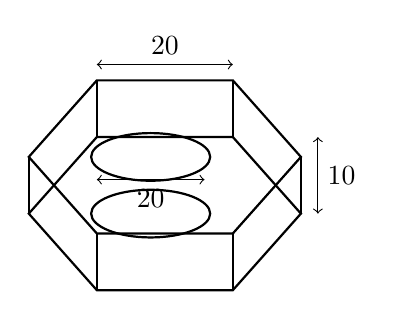
\begin{tikzpicture}[scale=0.72]
  \coordinate (A) at (0,0);
  \coordinate (B) at (2.4,0);
  \coordinate (C) at (3.6,1.35);
  \coordinate (D) at (2.4,2.7);
  \coordinate (E) at (0,2.7);
  \coordinate (F) at (-1.2,1.35);
  \coordinate (A') at (0,-1.0);
  \coordinate (B') at (2.4,-1.0);
  \coordinate (C') at (3.6,0.35);
  \coordinate (D') at (2.4,1.7);
  \coordinate (E') at (0,1.7);
  \coordinate (F') at (-1.2,0.35);
  \draw[thick] (A)--(B)--(C)--(D)--(E)--(F)--cycle;
  \draw[thick] (A')--(B')--(C')--(D')--(E')--(F')--cycle;
  \foreach \p/\q in {A/A',B/B',C/C',D/D',E/E',F/F'}
    \draw[thick] (\p)--(\q);
  \draw[thick] (0.95,1.35) ellipse [x radius=1.05, y radius=0.42];
  \draw[dashed] (0.95,1.35) ellipse [x radius=1.05, y radius=0.42];
  \draw[thick] (0.95,0.35) ellipse [x radius=1.05, y radius=0.42];
  \draw[dashed] (0.95,0.35) ellipse [x radius=1.05, y radius=0.42];
  \draw[<->] (0.0,2.98)--(2.4,2.98) node[midway,above] {$20$};
  \draw[<->] (3.9,0.35)--(3.9,1.7) node[midway,right] {$10$};
  \draw[<->] (0.0,0.95)--(1.9,0.95) node[midway,below] {$20$};
\end{tikzpicture}
\end{center}
\nopagebreak[4]
\begin{gktip}
原图在外六边形的一条边、圆孔和高度方向分别标出 $20$、$20$、$10$；下文若按通常六角螺帽构形解答，将其解释为外正六边形边长 $20\ \mathrm{mm}$、圆孔直径 $20\ \mathrm{mm}$、高度 $10\ \mathrm{mm}$。
\end{gktip}

\end{question}
\begin{question}
\gkti{6}求直线 $x+\sqrt3y+3\sqrt3=0$ 的斜率和倾角，并画出它的图形。

\end{question}
\begin{question}
\gkti{7}当 $x$ 为何值时，函数 $y=x^2-8x+5$ 的值最小，并求出这个最小值。

\end{question}
\begin{question}
\gkti{8}将浓度为 $96\%$ 和 $36\%$ 的甲、乙两种流酸配制成浓度为 $70\%$ 的流酸 $600$ 升，问应从甲、乙两种流酸中各取多少升？

\end{question}